\newpage
\section{Background\label{introduction:background}}

\subsection{Breast Cancer Overview\label{sec:introduction:breastcanceroverview}}
Breast cancer is a type of cancer that starts in one or both breasts. The left and right breast are each mainly glands, ducts, and fatty tissue. Breast cancer can start in these different parts of the breast or others~\cite{RefWorks:RefID:36-american2021breast}.

\subsubsection{Statistics\label{sec:introduction:breastcancer:statistics}}
Breast cancer accounts for about 30\% of all new cancer cases in U.S. women each year~\cite{RefWorks:RefID:150-2025breast}. The average risk of a woman in the U.S. developing breast cancer sometime in her life is about 1 in 8 (about 13\%)~\cite{RefWorks:RefID:36-american2021breast}. Breast cancer is also the second leading cause of cancer death in women behind lung cancer~\cite{RefWorks:RefID:36-american2021breast}.

\subsubsection{Development and Spread\label{sec:introduction:breastcancer:developmentandspread}}
Breast cancer can start in different parts of the breast, such as the ducts, lobules, or the tissue in between. The cancer can spread when cancer cells are carried to other parts of the body through blood or the lymphatic system. The lymphatic system is a network of small bean-sized glands called lymph nodes, ducts, and vessels that carry clear lymph fluid throughout the body. This clear lymph fluid contains immune system cells to fight infection as well as waste and tissue by-products. This system carries lymph fluid away from the breast; cancer cells can enter the lymph vessels, grow inside lymph nodes, and spread to other parts of the body~\cite{RefWorks:RefID:36-american2021breast}.

The most common areas where lymph vessels of the breast drain into are the underarm (axillary), inside the chest near the breastbone (internal mammary), and around the collar bone (supraclavicular and infraclavicular). Once cancer cells have spread to  the lymph nodes, there is a higher chance of metastases, or spreading, to other parts of the body which is called metastatic breast cancer~\cite{RefWorks:RefID:36-american2021breast}.

The method of cancer cells metastasizing through the lymphatic system is illustrated below in Figure~\ref{fig:introduction:lymphatic_system_in_a_breast} and Figure~\ref{fig:introduction:lymphatic_process_of_metastatic_breast_cancer}.

\begin{figure}[h!]
        \begin{minipage}{0.92\textwidth}
                \centering
                \begin{subfigure}[b]{0.45\textwidth}
                        \centering
                        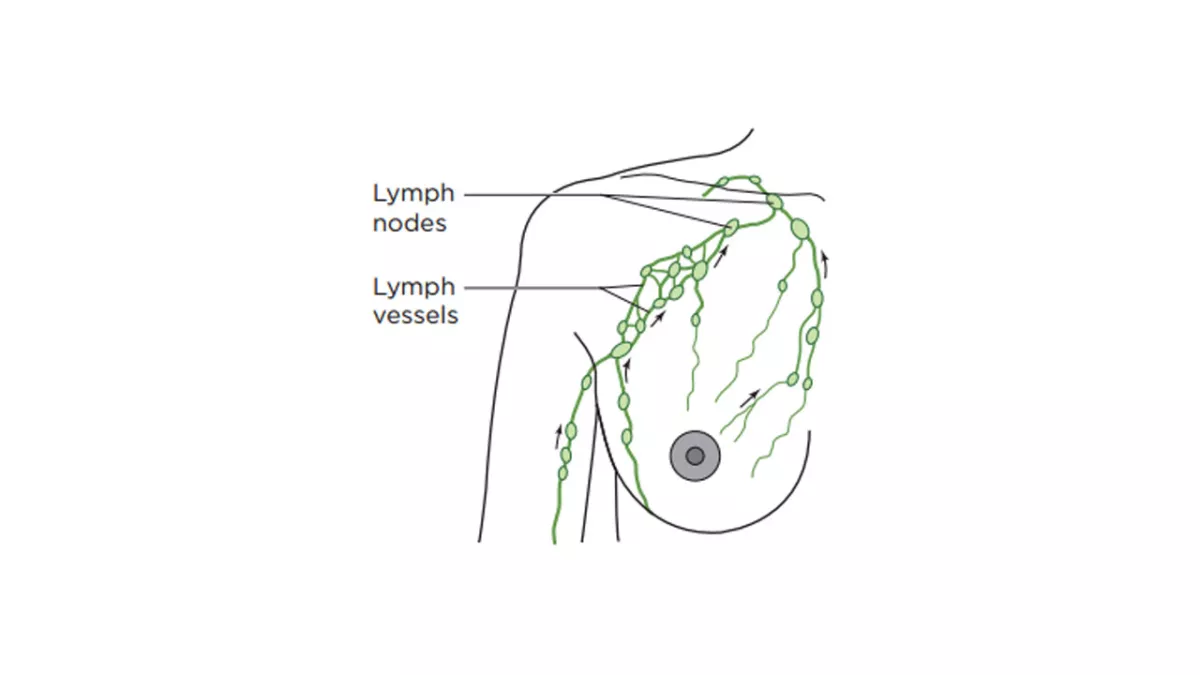
\includegraphics[width=\textwidth]{../figs/introduction/lymphatic_system_in_a_breast.png}
                        \caption{Lymphatic System Overview \cite{RefWorks:RefID:37-memorialsurgery}.}
                        \label{fig:introduction:lymphatic_system_in_a_breast}
                \end{subfigure}
                \begin{subfigure}[b]{0.45\textwidth}
                        \centering
                        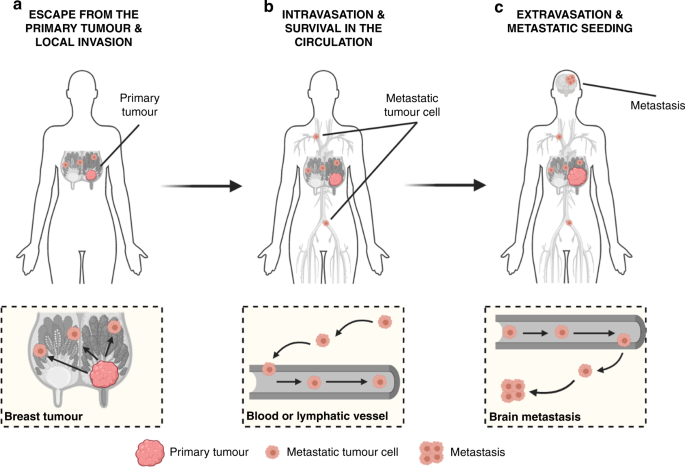
\includegraphics[width=\textwidth]{../figs/introduction/process_of_metastatic_breast_cancer.png}
                        \caption{Lymph Nodes Overview \cite{RefWorks:RefID:364-riggio2020lingering}.}
                        \label{fig:introduction:lymphatic_process_of_metastatic_breast_cancer}
                \end{subfigure}
        \end{minipage}
        \caption{Lymphatic System and Lymph Nodes Overview \cite{RefWorks:RefID:364-riggio2020lingering} \cite{RefWorks:RefID:37-memorialsurgery}.}
        \label{fig:introduction:lymphatic_system_and_nodes_overview}
\end{figure}

\subsection{Treatment of Breast Cancer\label{sec:introduction:treatmentofbreastcancer}}

\subsubsection{Stages of Breast Cancer\label{sec:introduction:breastcancer:stagesofbreastcancer}}
% Early vs late stage
Breast cancer is classified in stages ranging from 0 to IV based on the cancer's characteristics such as tumor size~\cite{RefWorks:RefID:151-2025breast}.

Stage 0 breast cancer is described as non-invasive, meaning the cancer cells are confined to the ducts or lobules in the breast and have not spread to surrounding healthy tissue~\cite{RefWorks:RefID:151-2025breast}.

Stage I breast cancer is invasive, meaning the cancer cells have spread to surrounding healthy tissue. In stage I breast cancer, the tumor is up to 2cm in size but invading cancer cells are no more than 1mm. Stage I is classified as either IA or IB depending on the sevarity of the cancer.~\cite{RefWorks:RefID:151-2025breast}.

Stage II breast cancer is used when the cancer is larger than 2cm but no larger than 5cm, or if the cancer has spread to one to three nearby lymph nodes. Similar to stage I breast cancer, stage II breast cancer can be subdivided into IIA and IIB~\cite{RefWorks:RefID:151-2025breast}.

Stage II breast cancer can be divided into IIIA, IIIB, and IIIC. This stage describes invasive breast cancer that is larger than 5cm or is found in four to nine nearby lymph nodes (IIIA), has spread to the chest wall or skin of the breast (IIIB), or has spread to ten or more nearby lymph nodes or to lymph nodes above or below the collarbone (IIIC)~\cite{RefWorks:RefID:151-2025breast}.

Lastly, stage IV breast cancer describes cancer that has metastasized, or spread, to other parts of the body such as the lungs, liver, bones, or brain~\cite{RefWorks:RefID:151-2025breast}.

Breast cancer stages can be divided into early and late stage breast cancer. Early-stage breast cancer incudes stages 0, I, and IIA while late-stage breast cancer includes stages IIB, III, and IV~\cite{RefWorks:RefID:365-stages}. Table~\ref{tab:introduction:breastcancer:stages} summarizes the stages of breast cancer. An overview of breast cancer treatment options for early and late stage breast cancer is shown in Figure~\ref{fig:introduction:breast_cancer_treatment_options_overview}.


\begin{table}[h!]
        \centering
        \caption{Stages of Breast Cancer~\cite{RefWorks:RefID:151-2025breast, RefWorks:RefID:365-stages}.}
        \label{tab:introduction:breastcancer:stages}
        \begin{tabular}{|c|c|c|}
                \hline
                \textbf{Stage} & \textbf{Description}                                       & \textbf{Early/Late Stage} \\
                \hline
                0              & Non-invasive, confined to ducts or lobules                 & Early                     \\
                \hline
                I              & Invasive, tumor up to 2cm, invading cells no more than 1mm & Early                     \\
                \hline
                IIA            & Tumor 2-5cm or spread to 1-3 lymph nodes                   & Early                     \\
                \hline
                IIB            & Tumor larger than 5cm or spread to 1-3 lymph nodes         & Late                      \\
                \hline
                IIIA           & Tumor larger than 5cm or found in 4-9 lymph nodes          & Late                      \\
                \hline
                IIIB           & Spread to chest wall or skin of breast                     & Late                      \\
                \hline
                IIIC           & Spread to 10+ lymph nodes or above/below collarbone        & Late                      \\
                \hline
                IV             & Metastasized to other parts of the body                    & Late                      \\
                \hline
        \end{tabular}
\end{table}

\subsubsection{Current Treatment Options\label{sec:introduction:breastcancer:currenttreatmentoptions}}

\paragraph*{Surgical Options\label{sec:introduction:breastcancer:currenttreatmentoptions:surgicaloptions}}

Treatment options for breast cancer largely depend on the type and stage of the cancer. Surgical choices include a lumpectomy, which removes the tumor and a small margin of surrounding healthy tissue, or a mastectomy, which removes the entire breast~\cite{RefWorks:RefID:165-czajka2023breast}.

A lumpectomy is followed by radiation therapy to kill any stray cancer cells that may remain in the breast. This combination helps lower the risk of recurrence, or the return of the cancer~\cite{RefWorks:RefID:159-depolo2024radiation}. Radiation therapy is performed using high-energy X-rays to damage a cancer cell's DNA, preventing it from dividing further until it dies. Healthy tissue cells grow and divide slower than cancer cells, allowing them to repair themselves after radiation therapy while cancer cells cannot~\cite{RefWorks:RefID:159-depolo2024radiation}. See Section~\ref{sec:introduction:radiationtherapy} for more information on radiation therapy.

\paragraph*{Lymph Node Biopsy\label{sec:introduction:breastcancer:currenttreatmentoptions:lymphnodebiopsy}}
In most surgical treatments for breast cancer, a lymph node biopsy is performed to check if cancer has spread past the breast tissue and to the lymph nodes. Samples from one or more lymph nodes are removed and examined under a microscope for cancer cells~\cite{RefWorks:RefID:37-memorialsurgery}. Standard practice was removing most of the lymph nodes in the underarm, called an axillary dissection. Today, a sentinel lymph node biopsy is more commonly performed to allow a faster recovery time~\cite{RefWorks:RefID:37-memorialsurgery}.

\paragraph*{Sentinel Lymph Node Biopsy\label{sec:introduction:breastcancer:currenttreatmentoptions:sentinellymphnodebiopsy}}
The sentinel lymph node is the first lymph node that breast cancer cells spread to after leaving the breast. In a sentinel lymph node biopsy, a radioactive tracer (often technetium-99m) and/or a blue dye is injected into the side of the tumor. The tracer(s) travel through the lymphatic system to the sentinel lymph node. The blue stain and radiotracer signal, found with a gamma probe, can be used to identify and excise this lymph node for examination under a microscope for cancer cells~\cite{RefWorks:RefID:37-memorialsurgery},~\cite{RefWorks:RefID:165-czajka2023breast}.

\paragraph*{Systemic Therapies\label{sec:introduction:breastcancer:currenttreatmentoptions:systemictherapies}}
While breast cancer treatment commonly starts with surgery, systemic therapies such as chemotherapy, hormone therapy, or targeted therapies may also be used~\cite{RefWorks:RefID:37-memorialsurgery}.

Chemotherapy, often called "chemo," uses strong medicines to slow or stop cancer cells from growing further. As chemotherapy often works by attacking cells that divide quickly, it can attack cancer cells but also other healthy cells that divide quickly such as those that make your hair grow. This can lead to side effects such as hair loss and nausea~\cite{RefWorks:RefID:37-memorialsurgery}.

Hormone treatment is used for breast cancer cells that require hormones such as estrogen to grow. This is done by blocking the hormones these cancer cells need to grow. Side effects can include changes in menstrual cycle, hot flashes, and aching bones~\cite{RefWorks:RefID:37-memorialsurgery}.

Targeted therapies, or precision medicines, attack specific characteristics of an individual's cancer cells rather than attacking all rapidly dividing cells like chemotherapy. Targeted therapies can treat the most common breast cancer gene mutations such as BRCA1 and BRCA2, HER2, and PIK3CA. This individualized treatment can lead to less side effects than in chemotherapy~\cite{RefWorks:RefID:37-memorialsurgery}.

\begin{figure}[h!]
        \centering
        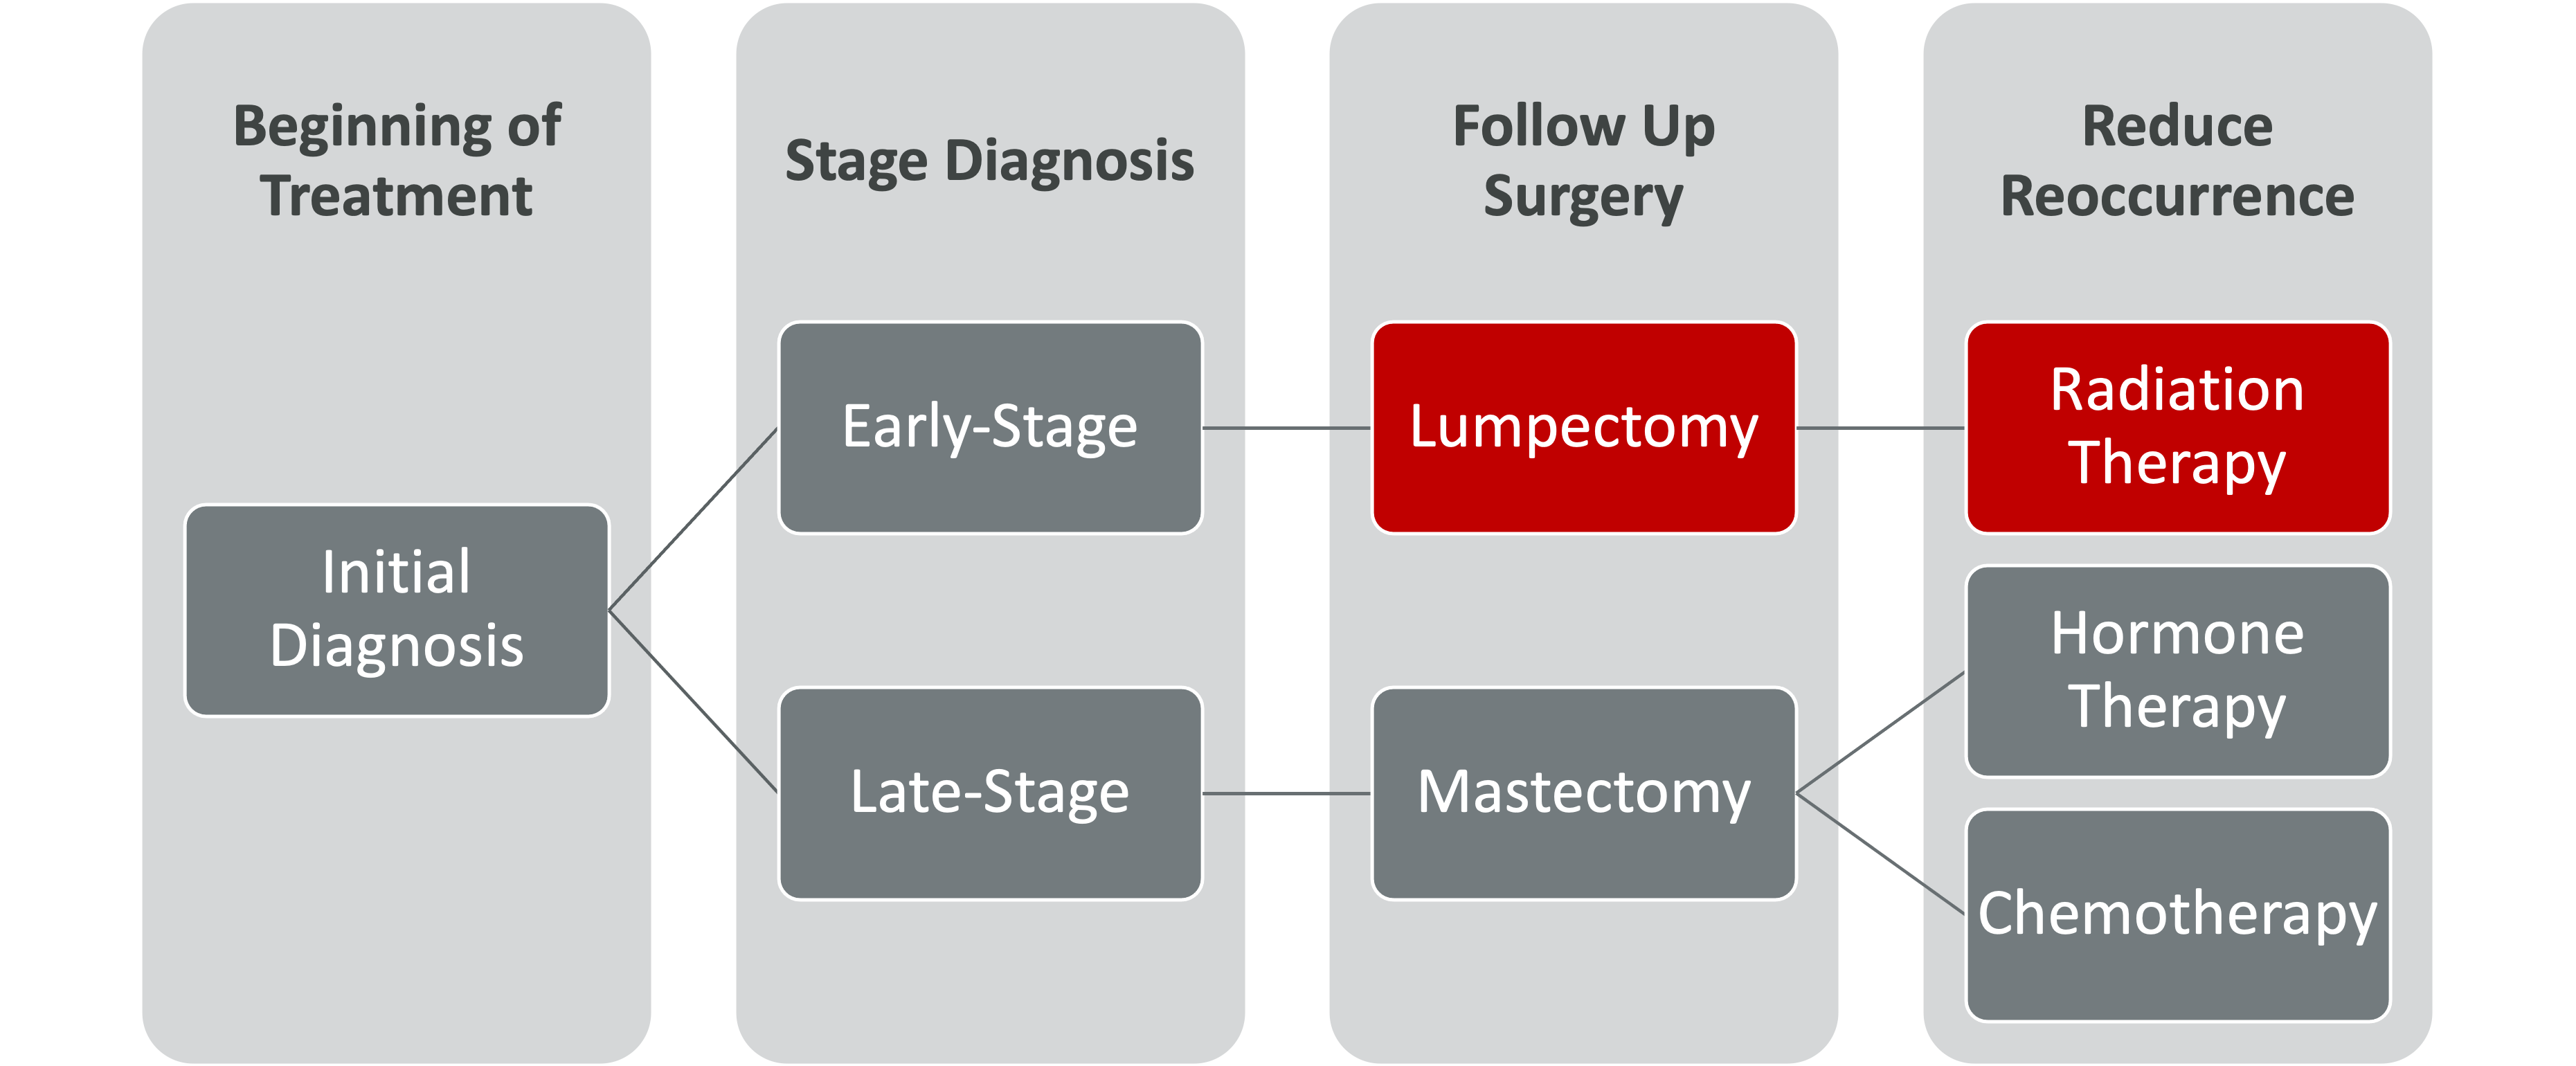
\includegraphics[width=\textwidth]{../figs/introduction/breast_cancer_treatment_process_flowchart.png}
        \caption{Breast Cancer Treatment Options Overview \cite{RefWorks:RefID:37-memorialsurgery}, \cite{RefWorks:RefID:370-einsteinisaac}.}
        \label{fig:introduction:breast_cancer_treatment_options_overview}
\end{figure}

\subsection{Radiation Therapy\label{sec:introduction:radiationtherapy}}
\subsubsection{Radiation Therapy Overview\label{sec:introduction:radiationtherapy:overview}}
As mentioned in Section~\ref{sec:introduction:breastcancer:currenttreatmentoptions:surgicaloptions}, radiation therapy often follows a lumpectomy procedure to kill any stray cancer cells and prevent the cancer from resurfacing. Together, a lumpectomy procedure followed by radiation therapy is commonly known as breast-conserving therapy (BCT). Some compare breast cancer surgery to picking up the large pieces of a broken glass off the floor, while radiation therapy is like vacuuming the remaining shards at the end.

Including radiation therapy after a lumpectomy has been shown to reduce the risk of ipsilateral (same side) recurrence as well as increase overall survival rates~\cite{RefWorks:RefID:157-thomasscience}~\cite{RefWorks:RefID:198-jiao2024interobserver}~\cite{RefWorks:RefID:375-joosten2013evaluation}.

\subsubsection{Whole vs Accelerated Partial Breast Irradiation\label{sec:introduction:radiationtherapy:wholevsacceleratedpartialbreastirradiation}}
Patients undergoing BCT can receive either whole breast irradation (WBI) or accelerated partial breast irradiation (APBI). WBI is the more common of the two techniques, although APBI has been gaining traction in recent years due to its unique benefits~\cite{RefWorks:RefID:157-thomasscience}.

WBI is delivered over the course of five to six weeks while APBI is delivered over the course of one week. APBI also limits radiation exposure to 1-2 cm margin of healthy tissue surrounding the tumor site. This limited exposure reduces radiation exposure risks to surrounding organs such as lungs, heart, or ribs. APBI also resulted in higher rates of "excellent/good" cosmetic outcomes compared to WBI (81\% vs 63\% respectively)~\cite{RefWorks:RefID:157-thomasscience}. Comparison of radiation exposure in WBI vs APBI is illustrated in Figure~\ref{fig:introduction:WBI_vs_APBI_irradiation_comparison}.

\begin{figure}[h!]
        \centering
        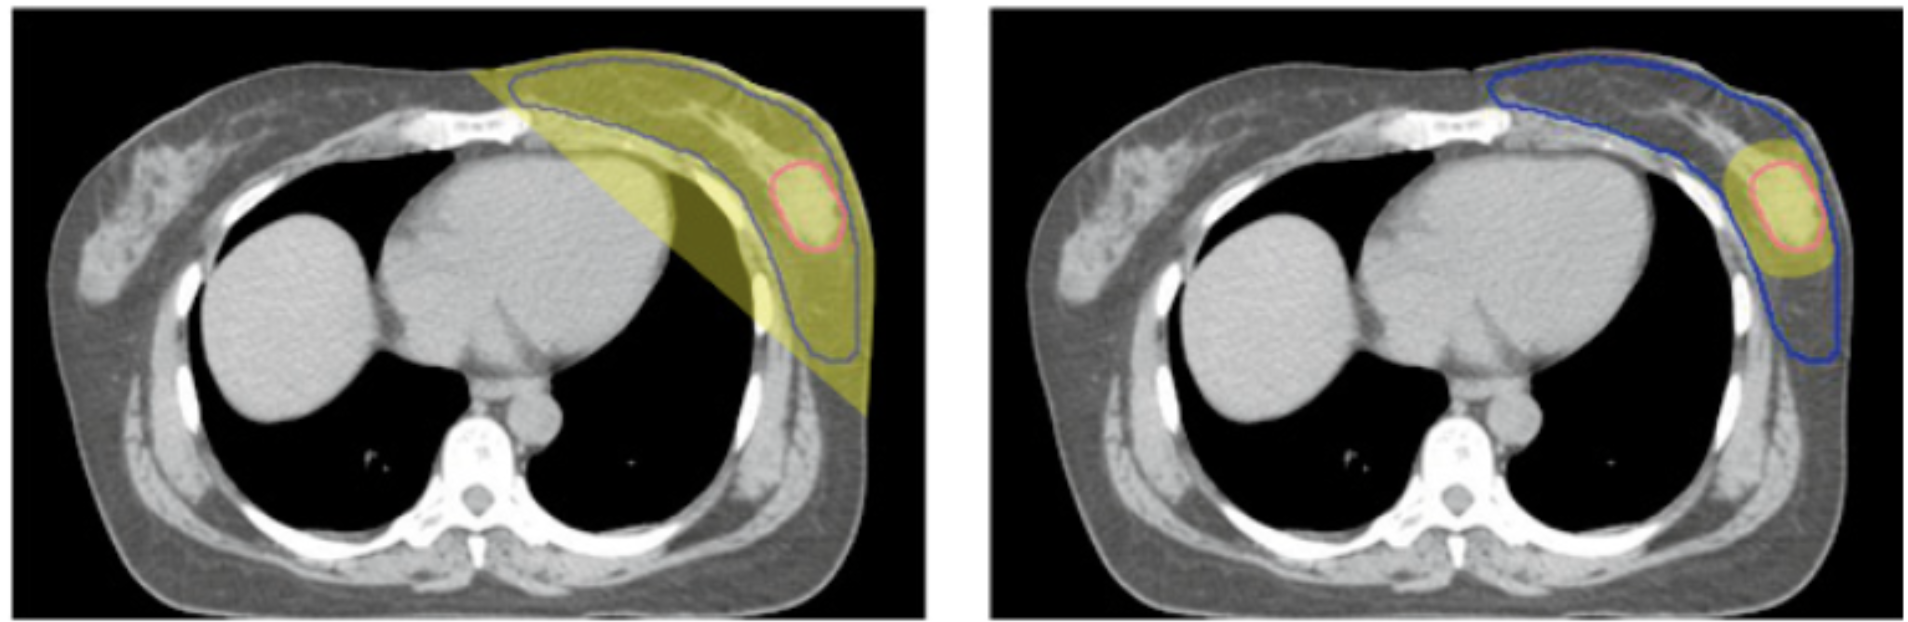
\includegraphics[width=0.8\textwidth]{../figs/introduction/WBI_vs_APBI_irradiation_comparison.png}
        \caption{Comparison of radiation exposure between Whole Breast Irradiation (WBI) (left) and Accelerated Partial Breast Irradiation (APBI) (right) \cite{RefWorks:RefID:157-thomasscience}. The yellow area indicates the irradiated region.}
        \label{fig:introduction:WBI_vs_APBI_irradiation_comparison}
\end{figure}

\subsubsection{Radiation Therapy Treatment Planning\label{sec:introduction:radiationtherapy:treatmentplanning}}

\paragraph*{Whole vs Partial Breast Irradiation\label{sec:introduction:radiationtherapy:treatmentplanning:WBIvsPBI}}
Radiation therapy (WBI or APBI) requires tumor bed delineation to identify and outline the tumor as well as a surrounding healthy tissue margin. This treatment planning ensures radiation is delivered accurately to the tumor site while minimizing exposure to healthy surrounding tissue and organs~\cite{RefWorks:RefID:197-den2015postlumpectomy}.

One concern with tumor bed (TB) delineation is the interobserver variability in accurately marking the TB~\cite{RefWorks:RefID:197-den2015postlumpectomy},~\cite{RefWorks:RefID:179-yang2013tumor}. There are many methods and devices used to assist in TB delineation to address these concerns such as surgical clips, pre-operative imaging, seroma formation, fiducial markers, and other implantable devices~\cite{RefWorks:RefID:179-yang2013tumor},~\cite{RefWorks:RefID:25-acree2022review}.

\paragraph*{Treatment Planning Volumes\label{sec:introduction:radiationtherapy:treatmentplanning:planningVolumes}}
% Ref 190:
The treatment planning volumes are divided into three sub-volumes: the gross target volume (GTV), the clinical target volume (CTV), and the planning target volume (PTV).

The GTV is the confirmed tumor based on visible or radiological examination. This is delineated based on clinical judgment~\cite{RefWorks:RefID:190-antolakplanning}.

The CTV encompasses the GTV with a margin for subclinical disease. Subclinical disease is an illness that is not clinically detectable but will show signs and symptoms after they surface~\cite{RefWorks:RefID:373-stöpplermedical}. Like the GTV, the CTV is also determined largely by clinical decisions, though it can be aided by computer software tools~\cite{RefWorks:RefID:190-antolakplanning}.

The PTV encompasses the CTV with a margin for uncertainty due to organ mobility, organ deformation, and variations in patient setup. The PTV is the target volume that receives radiation during radiation therapy. Once the CTV is delineated, the PTV can be created automatically using software tools. There is debate regarding the necessary margin size for CTV and PTV creation~\cite{RefWorks:RefID:190-antolakplanning}.

The differences between these three margins is illustrated below in Figure~\ref{fig:introduction:treatment_target_volumes_comparison}.
\begin{figure}[h!]
        \centering
        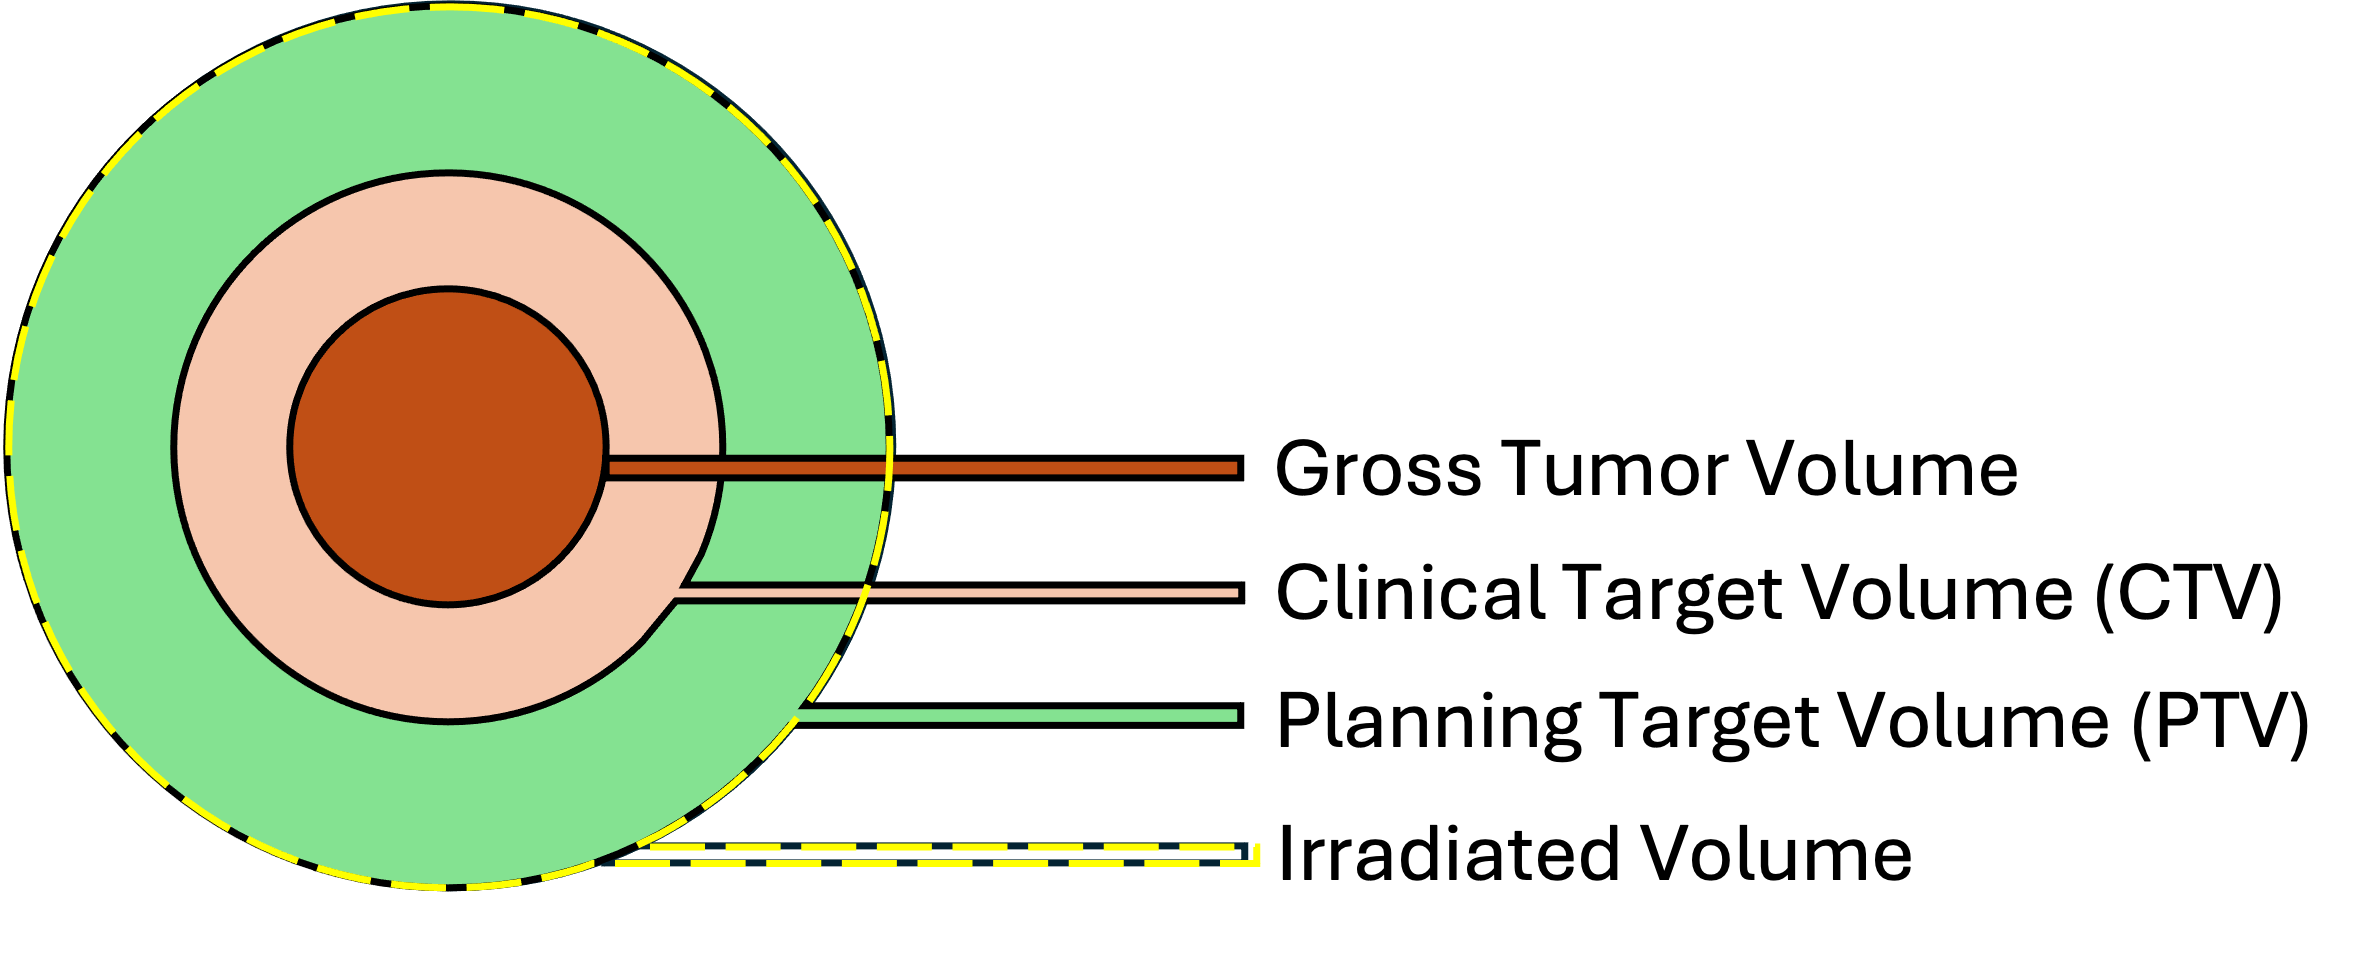
\includegraphics[width=0.8\textwidth]{../figs/introduction/treatment_target_volumes.png}
        \caption{Difference between radiation therapy treatment target volumes (GTV, CTV, and PTV). Adapted from~\cite{RefWorks:RefID:370-einsteinisaac}.}
        \label{fig:introduction:treatment_target_volumes_comparison}
\end{figure}


\subsection{Motivation\label{sec:introduction:motivation}}
The motivation for this work stems from the need to standardize and improve the accuracy and consistency of tumor bed (TB) delineation in radiation therapy following a lumpectomy procedure.

The challenges with accurate TB delineation following a lumpectomy procedure arise because the cancerous tissue has been removed, leaving behind a tumor cavity that is difficult to accurately trace~\cite{RefWorks:RefID:25-acree2022review}. Additionally, unlike other parts of the body, the breast lacks anatomic landmarks to assist with tumor bed delineation~\cite{RefWorks:RefID:344-mitchell2019adaptable}. This need for a marking method is visualized below in Figure~\ref{fig:introduction:need_for_tumor_bed_marker}. These challenges have been shown to lead to significant interobserver variability amongst radiation oncologists when marking TB volumes~\cite{RefWorks:RefID:191-kader2008ctbased}~\cite{RefWorks:RefID:194-kirby2013tumour}. To address this variability, one study explored the use of artificial intelligence (AI) to standardize the TB delineation process~\cite{RefWorks:RefID:195-poortmans2019winter}.

\begin{figure}[h!]
        \centering
        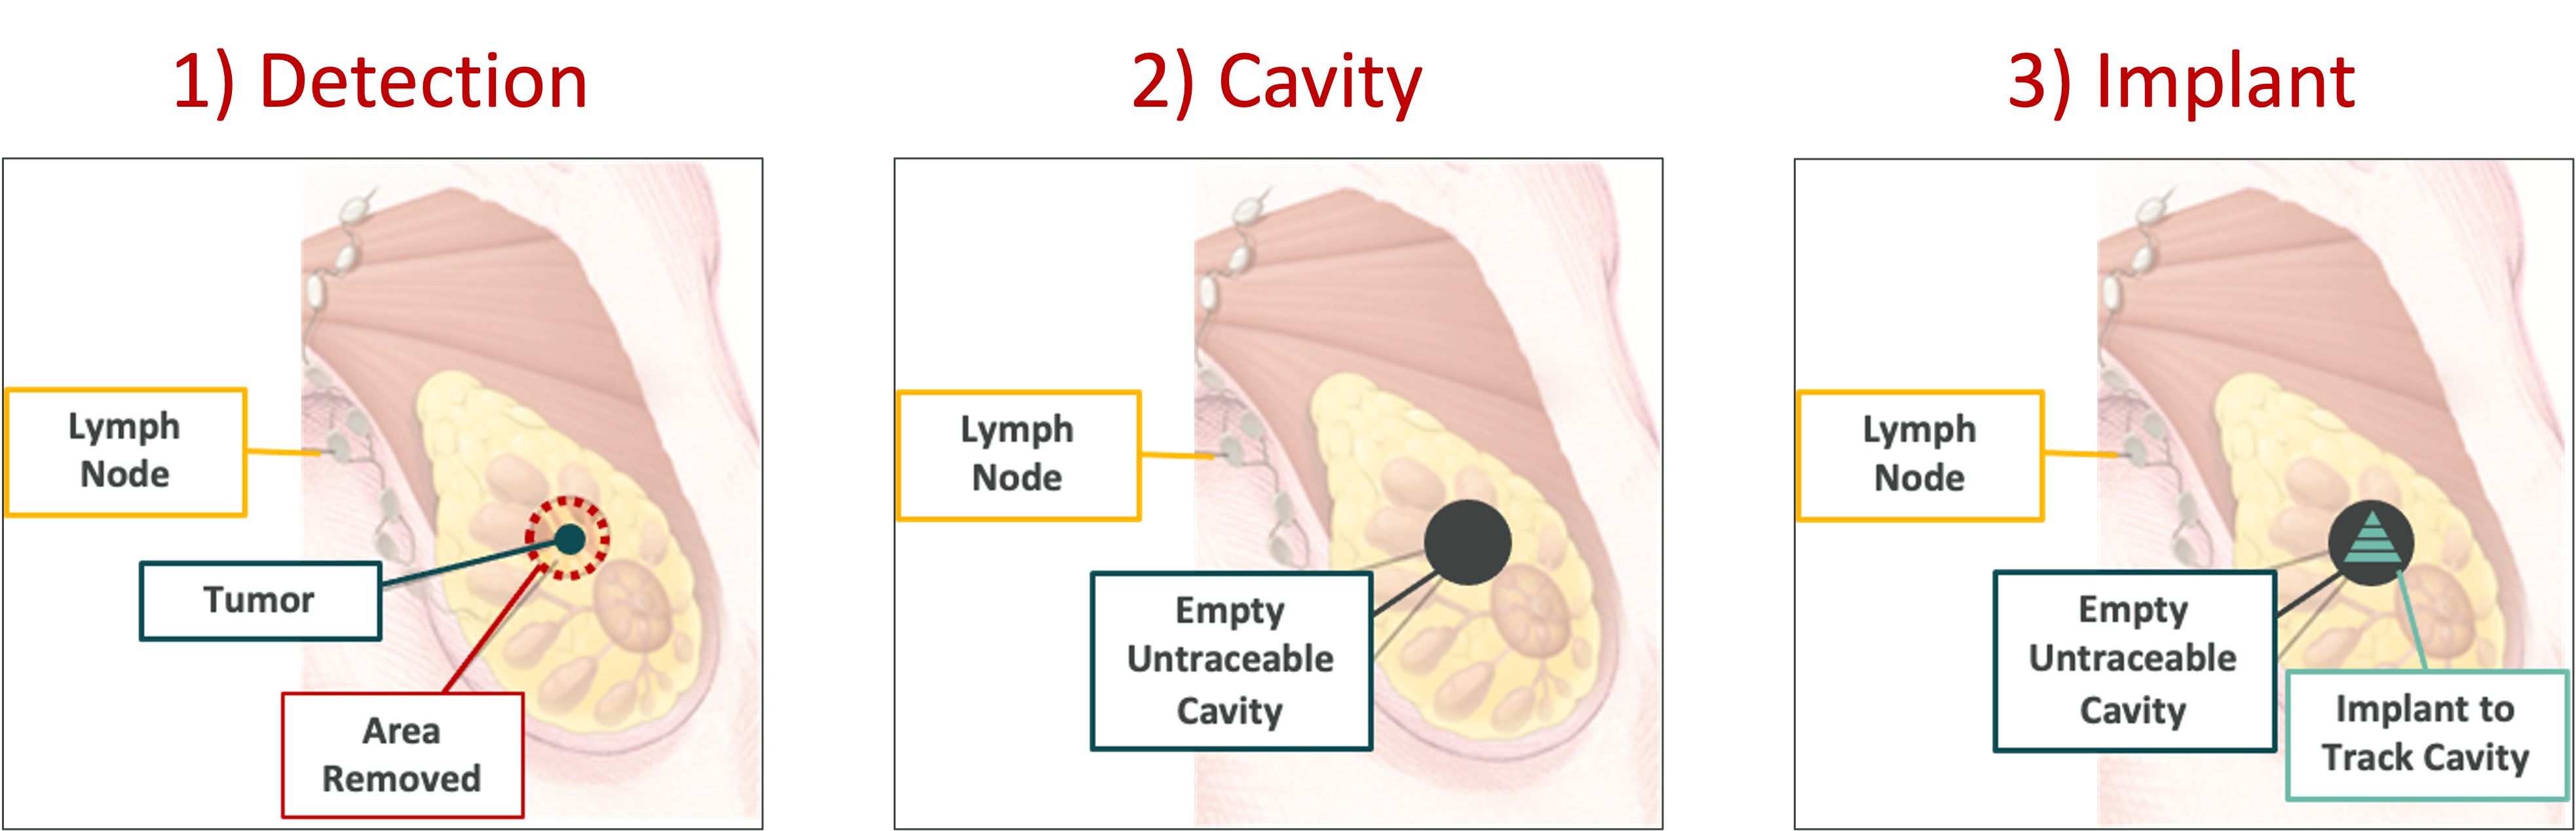
\includegraphics[width=\linewidth]{../figs/introduction/need_for_tumor_bed_marker.png}
        \caption{Motivation for tumor cavity marker following lumpectomy procedure. Adapted from \cite{RefWorks:RefID:38-johnbreastconserving}.}
        \label{fig:introduction:need_for_tumor_bed_marker}
\end{figure}

Current devices and methods used for TB delineation have limitations that affect the overall consistency and accuracy of post-lumpectomy radiation therapy. As over 70\% of breast cancer recurrences occur at the original tumor site, accurate TB delineation and radiation delivery is important in improving patient outcomes~\cite{RefWorks:RefID:25-acree2022review}.

% Current Devices
\subsubsection{Current Devices and Treatment Methods\label{sec:introduction:motivation:currentDevicesAndMethods}}
While this topic will be further explored in Section ~\ref{sec:literatureReview:currentMethods}, this section provides a brief overview of current treatment methods for radiation therapy planning.

There is no standardized protocol for TB delineation. Current methods and devices used for TB volume delineation include basing volumes on clinical notes, lumpectomy scars, seroma formation, fiducial clips/markers, and implantable devices such as Biozorb or Veraform~\cite{RefWorks:RefID:25-acree2022review}. Each of these methods have noted drawbacks creating opportunity for improvement in this area (see Section~\ref{sec:literatureReview:currentMethods:challengeswithcurrentdevicesandmethods})

A brief overview of these methods is shown below in Figure~\ref{fig:introduction:current_devices_overview}.

\begin{figure}[h!]
        \centering
        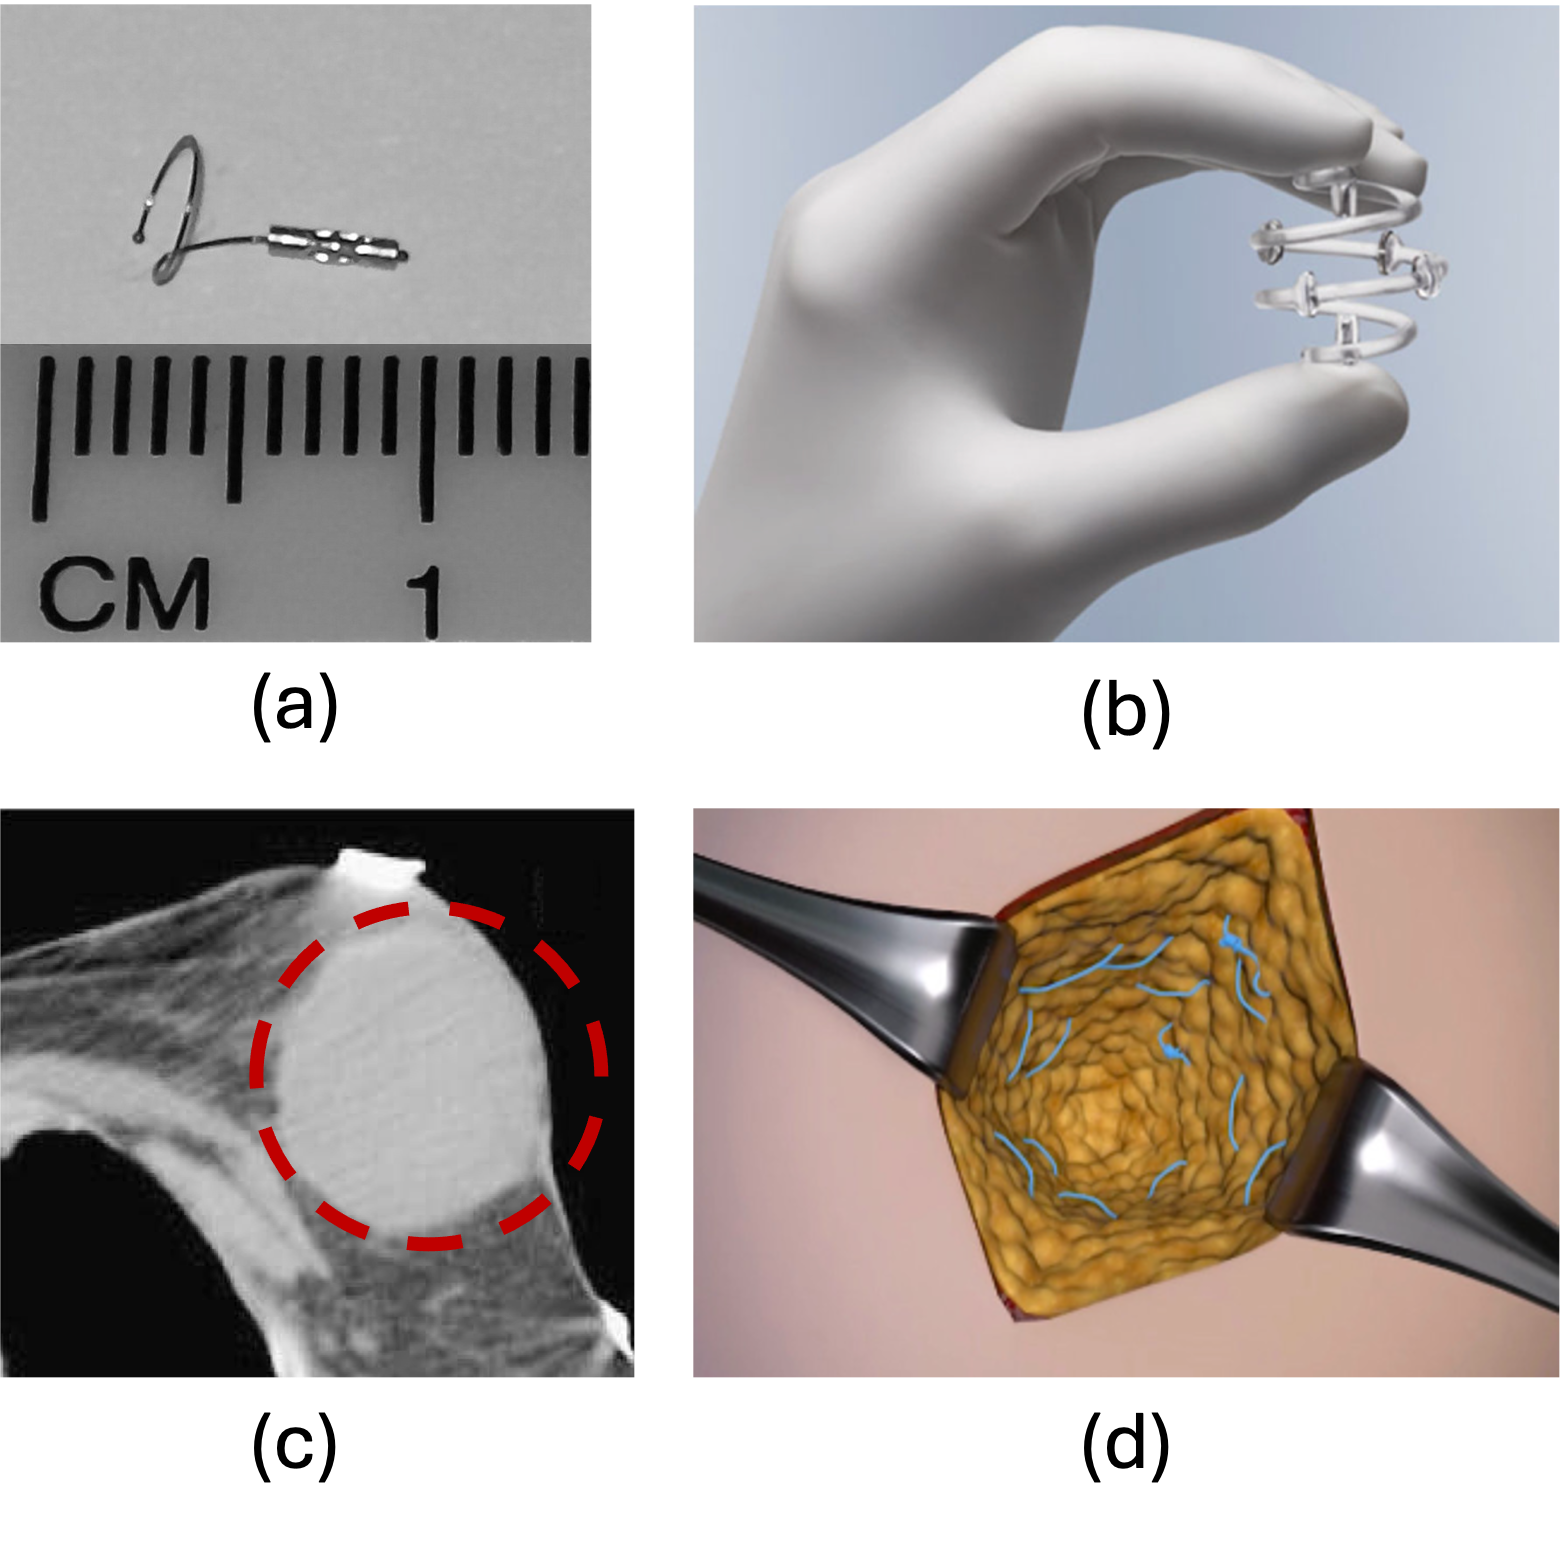
\includegraphics[width=0.6\linewidth]{../figs/introduction/current_devices_overview.png}
        \caption{Overview of Current TB Volume Marking Devices and Methods. Fiducial Clips (a), Biozorb (b), Seromas (c), and Veraform (d).}
        \label{fig:introduction:current_devices_overview}
\end{figure}

\subsubsection{Importance of Accurate Tumor Bed Delineation\label{sec:introduction:motivation:importanceofaccuratetumorbeddelineation}}

For breast cancer, TB delineation is largely based on Accurate TB delineation is crucial in effective radiation therapy following a lumpectomy procedure given the increasing use of APBI. Since APBI targets a small area of tissue surrounding the tumor bed, accurate delineation is necessary to ensure the radiation dose is delivered precisely to the intended area while minimizing exposure to surrounding healthy tissue and organs~\cite{RefWorks:RefID:197-den2015postlumpectomy}, ~\cite{RefWorks:RefID:25-acree2022review}.

Overestimating TB volume, common in seroma-based delineation, is associated with an increased risk of subcutaneous fibrosis and poorer cosmetic results~\cite{RefWorks:RefID:197-den2015postlumpectomy}. Conversely, underestimating TB volume can lead to insufficient radiation coverage of the tumor bed, increasing the risk of local recurrence~\cite{RefWorks:RefID:198-jiao2024interobserver}. An inaccurate TB volume can
also lead to alteration of management of a radiation boost and completely missing one or more margins of the TB~\cite{RefWorks:RefID:344-mitchell2019adaptable}.

\subsubsection{Proposed Solution\label{sec:introduction:motivation:proposedsolution}}
% Explain our research and the proposed mesh
Improving on shortcomings of existing tumor bed marking methods and devices (see \ref{sec:literatureReview:currentMethods}), it was hypothesized that an ideal device would need to be continuously radiopaque, biodegradable, and minimalistic.

It was determined that the ideal way to achieve these goals is through a thin flexible mesh made up of a biodegradable material with an embedded radiopaque agent~\cite{RefWorks:RefID:372-krakovskytumor}. The first iteration of this device is shown below in Figure~\ref{fig:introduction:initialCapstonePrototype}. This thesis details the prior and ongoing work to further develop this concept.

\begin{figure}[h!]
        \centering
        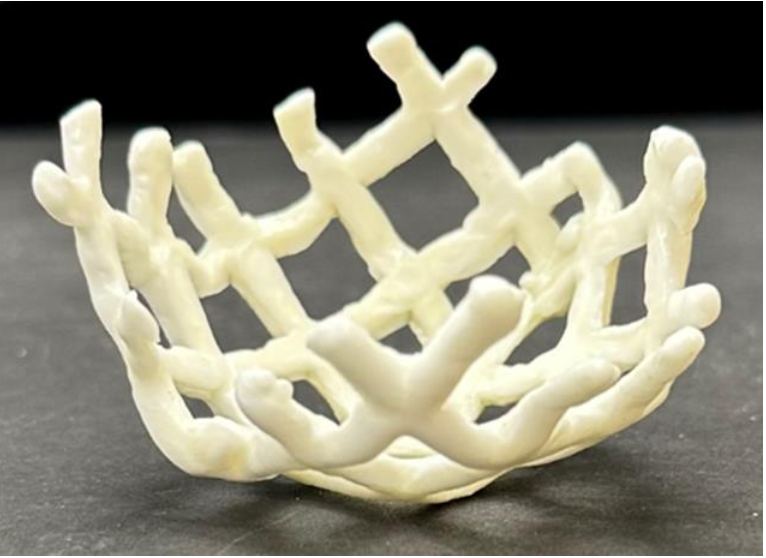
\includegraphics[width=0.6\linewidth]{../figs/introduction/initial_capstone_prototype.png}
        \caption{Initial prototype of proposed radiopaque biodegradable mesh implant~\cite{RefWorks:RefID:372-krakovskytumor}.}
        \label{fig:introduction:initialCapstonePrototype}
\end{figure}
